\chapter{Conclusioni}
\label{cap:chapter8}

\section{Obiettivi raggiunti}

A conclusione del tirocinio, il candidato è riuscito a raggiungere gli obiettivi preposti, sviluppando così un sistema che fosse in grado di fornire e far visualizzare le mappe richieste.
\\Il tirocinante ha infatti iniziato estendendo con successo il componente Angular delle mappe (lato front-end), integrando al suo interno tutti i protocolli OGC richiesti per la trasmissione dei dati geospaziali e ha realizzato una parte all'interno dell'applicazione web che permettesse di testare il funzionamento di tali protocolli, riuscendo a far visualizzare con successo diverse mappe (almeno una per ogni protocollo) e a rappresentarle correttamente nelle loro rispettive proiezioni.
\\Successivamente, ha introdotto nell'applicazione un software con lo scopo di fungere da server di mappe, chiamato GeoServer, il quale è stato utilizzato per la gestione e la distribuzione di questi dati. Nello specifico, ciò ha permesso di memorizzare sia i file locali in formato Shapefile (con i rispettivi file di stile in formato SLD), sia di effettuare proxying dei server OGC esterni, riuscendo anche a fornirli mediante protocollo WMTS, sebbene questi ultimi non lo supportassero. In aggiunta, dopo aver abilitato i suoi meccanismi di cache interna e grazie ai meccanismi di caching configurati nel WebServer (in quanto Reverse Proxy), è stato così possibile risolvere i problemi di rate-limiting e di lentezza riscontrati durante il proxying ai server esterni. 
\\Inoltre, il candidato si è proposto di sviluppare un nuovo programma, noto con il nome di AutoLoader, il quale ha permesso di caricare in automatico tutte le mappe all'interno di GeoServer. Ciò è stato ritenuto necessario dal tirocinante poiché tale procedura risultava molto laboriosa e complessa da effettuare manualmente, sopratutto considerato l'elevato numero di mappe da dover inserire. Per fare ciò, si è fatto uso delle API fornite da GeoServer stesso, le quali, sfortunatamente, non erano state aggiornate dagli sviluppatori con l'evoluzione del software. Il candidato ha quindi dovuto testare manualmente, per ogni richiesta HTTP necessaria, il suo vero funzionamento, così da poter modificare il modo in cui il programma AutoLoader inviava e riceveva le richieste da GeoServer.
\\Infine, è stato poi realizzato un ulteriore programma, lato back-end, il quale ha memorizzato all'interno di un database l'elenco di tutte le mappe disponibili, specificando per ognuna di esse: il nome della mappa, la categoria (rischio frane, alluvioni, etc...) e il modo in cui doveva contattare il server di mappe per reperire il dato, indicandone anche il protocollo OGC da utilizzare. Tutto ciò è stato infine reso disponibile attraverso una Rest API, così da poter esporre tutte queste informazioni al di fuori del back-end. 
\\Successivamente, il candidato ha realizzato un'altra pagina web in grado di contattare il servizio di Rest API, così da richiedere l'elenco di mappe disponibili e, ha reso questa lista visualizzabile all'utente, in modo che potesse selezionare le mappe ed interagire con le stesse.
\medskip
\\Nell'immagine \ref{fig:BMSArchitectureSequenceDiagram} è presente un diagramma di sequenza che espone il funzionamento di tutta l'architettura implementata durante l'intero percorso di tirocinio: essa mostra i passaggi che vengono eseguiti quando un utente accede all'applicazione per richiedere l'elenco di mappe.
\begin{figure}[htbp]
      \centering
      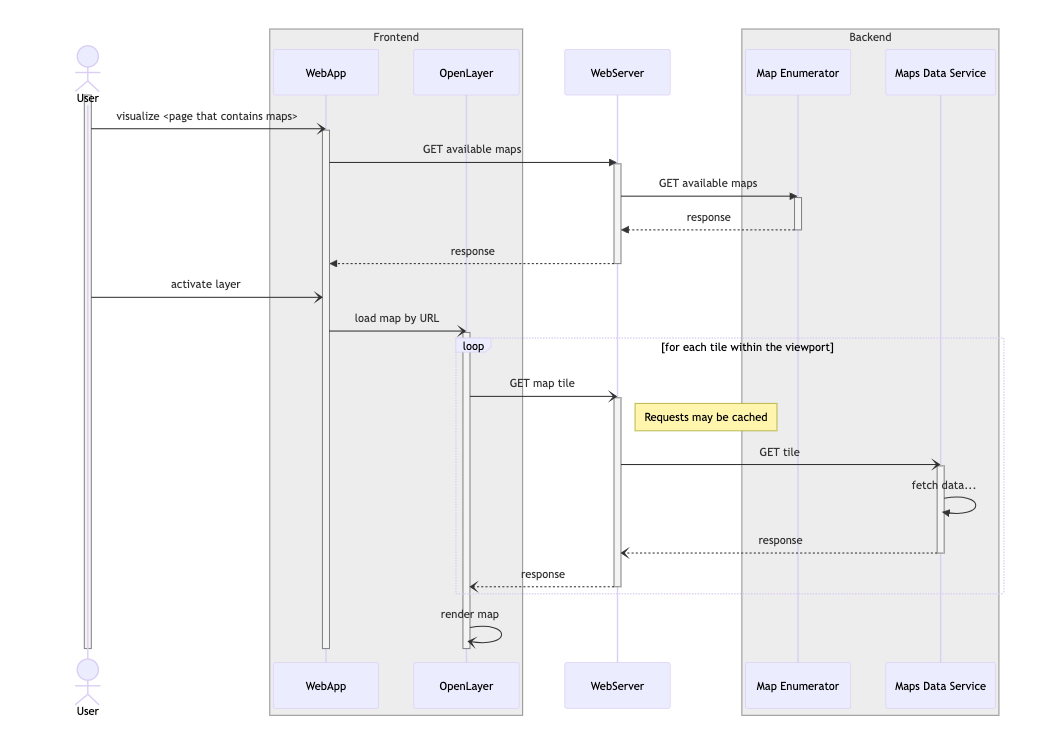
\includegraphics[width=1\textwidth]{Tesi/images/Capitolo8/BMSArchitectureSequenceDiagram.jpg}
      \caption{Diagramma di sequenza che illustra l'architettura realizzata}
      \label{fig:BMSArchitectureSequenceDiagram}
\end{figure}
\\Il client inizia la sua esecuzione inviando una richiesta HTTP al WebServer per ottenere l'elenco completo delle mappe disponibili. Il WebServer, in quanto Reverse Proxy, agisce come intermediario ed inoltra tale richiesta al servizio di Rest API. Una volta ottenuta la risposta, il WebServer la trasmette al client. A questo punto l'interfaccia web dell'applicazione è in grado di visualizzare la lista delle mappe disponibili.
\\Successivamente, una volta che l'utente ha selezionato una mappa specifica, il client, avendo già accesso a tutte le informazioni necessarie, invia una o più richieste HTTP al WebServer, le quali sono formulate in base al tipo di protocollo OGC scelto (per semplificare il diagramma di sequenza, viene mostrato solamente il protocollo WMTS).
Il WebServer, a sua volta, inoltra tali richieste al server di mappe per ottenere i dati richiesti. Dopo aver ottenuto le risposte desiderate, quest'ultimo risponde inviando i dati al WebServer, che a sua volta li trasmette al client. Adesso il client è in grado di visualizzare l'immagine della mappa selezionata. Come viene descritto anche all'interno del diagramma, l'utilizzo del WebServer permette di eseguire caching fra le varie richieste HTTP che vengono inviate.

\section{Riflessioni su sviluppi futuri}

In conclusione, sebbene l'applicazione risulti funzionante, ciò che è stato sviluppato durante il percorso di tirocinio rimane comunque un prototipo. Alla fine del progetto, le mappe non erano ancora state rese disponibili per un ambiente di produzione, in quanto non è ancora stata predisposta una struttura apposita che le possa ospitare. Infatti, le mappe venivano solamente caricate all'interno di un'istanza di GeoServer locale, eccetto durante le presentazioni di alcune demo, in cui veniva utilizzato un server dell'azienda. Inoltre, non era presente alcun meccanismo che permettesse di fornire una mappa proveniente da un server esterno, se quest'ultimo dovesse risultare momentaneamente non disponibile. Durante il periodo di tirocinio, infatti, è accaduto più volte che i servizi esterni andassero in manutenzione o smettessero di funzionare per un lungo periodo di tempo, rendendo così alcune mappe dell'applicazione momentaneamente inutilizzabili. 
\\Per risolvere questo problema, si potrebbe realizzare un meccanismo simile a quello proposto dal candidato precedentemente, sfruttando anche in questo caso le funzionalità offerte da GeoServer. Infatti, oltre ad effettuare proxying dei server esterni, si potrebbe configurare questo software affinché funzioni come mirror, ovvero scarichi localmente tutti i dati ricevuti, così da poter evitare di contattare dei servizi esterni all'azienda. Chiaramente questo meccanismo necessiterebbe di una struttura apposita che sia in grado di ospitare una grande mole di dati, in quanto, come già spiegato precedentemente, il peso dei dati geospaziali può risultare molto elevato.  Un'altra funzionalità che si potrebbe integrare è il supporto al protocollo TMS, il quale, come già ampiamente illustrato all'interno della relazione, potrebbe offrire in alcuni casi delle prestazioni migliori rispetto agli altri protocolli utilizzati; oltre che a offrire una struttura di archiviazione delle tiles, ottimale per l'uso dei servizi Amazon storage S3 e CDN CloudFront. Si potrebbe quindi utilizzare un sistema di servizi Cloud (come AWS) che permetta di supportare tale infrastruttura, archiviando direttamente al loro interno le immagini delle tiles, rappresentanti le mappe. Ciò comporterebbe un aumento delle prestazioni, in modo che il client richieda tramite protocollo TMS (dove possibile) le immagini a tiles, contattando direttamente questi servizi, i quali possono essere scalati in caso di necessità. In aggiunta, poiché l'intera applicazione è stata realizzata utilizzando container Docker, si potrebbe, ove necessario, scalare le loro istanze sia verticalmente, aumentando la potenza di calcolo del singolo servizio, che orizzontalmente, aumentando il numero di istanze contemporanee del servizio stesso. Ciò permetterebbe, ad esempio, di poter aumentare il numero di servizi in parallelo di GeoServer, riuscendo, in caso di necessità, ad ottenere una trasmissione più efficiente dei dati geospaziali mediante i protocolli così implementati.
